\section*{\huge \textcolor{Red}{ Bayesian Inference } \small \textit{ Suy luận Bayes } }
Tham khảo: \footnote{ \url{https://vi.wikipedia.org/wiki/Suy_lu\%E1\%BA\%ADn_Bayes} }
\subsection*{Định nghĩa:}
Suy luận Bayes là một kiểu suy luận thống kê mà trong đó các quan sát hay bằng chứng được dùng để cập nhật hoặc suy luận ra xác suất cho việc một giả thuyết có thể là đúng.

\section*{\huge \textcolor{Red}{ Bias term } \small \textit{ Hệ số điều chỉnh, Độ chệch } }
Tham khảo: \footnote{ \url{https://viblo.asia/p/khi-tat-ca-cac-phan-tich-hoc-may-deu-da-loi-thoi-overfitting-khong-ton-tai-XL6lAvDg5ek} }
\subsection*{Định nghĩa:}
Hệ số điều chỉnh, độ chệch là sự sai khác giữa trung bình dự đoán của mô hình chúng ta đang xây dựng với giá trị chính xác để dự đoán.
\begin{{figure}}[!h]
	\centering
	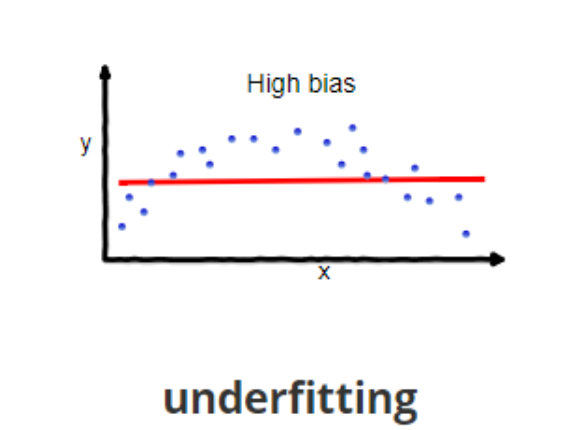
\includegraphics[width=0.5\linewidth]{ figures/B_Bias_NCB_N1.png }
	\caption{ Ví dụ về độ chệch trong bài toán hồi quy tuyến tính. }\label{fig:bias term_1}
\end{figure}

